\section{Literature Review}
\begin{frame}{Literature Review}
\framesubtitle{Beyond Monetary Transactions}
Blockchain has been studied as a tool for preserving non-monetary information by Lemieux~\cite{Lemieux2016Trusting}.\\
\vspace*{0.2cm}
Shows that public blockchains can provide integrity guarantees for the preservation of digital records.\\
\vspace*{0.2cm}
\begin{block}{Remark}
Blockchain preserves record integrity, but does not guarantee record correctness or long-term archival reliability, since its security relies on hash functions and digital signatures whose strength may change over time.
\end{block}
\end{frame}

\begin{frame}{Literature Review}
    \framesubtitle{Data Anchoring in Bitcoin}
Bitcoin allows arbitrary data to be embedded within transaction structures.\\
Gao~\cite{Gao2017Decentralized},proposes anchoring information by encoding data into fake P2PKH addresses.\\
\vspace*{0.2cm}
\hspace*{0.25cm}
{\centering 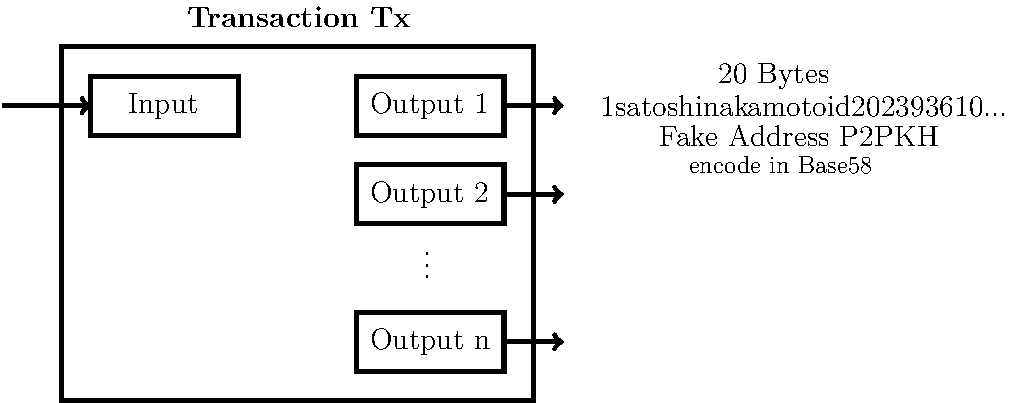
\includegraphics[scale=0.5]{figures/tx.pdf}\\}
\vspace*{0.2cm}
The method permanently burns Bitcoin, making it economically inefficient.
\end{frame}

\begin{frame}{Literature Review}
    \framesubtitle{Data Anchoring in Bitcoin}

Bartoletti et al.~\cite{Bartoletti2019BitcoinMetadata} analyze data embedding techniques in Bitcoin and highlight their impact on the UTXO set and node performance.\\
\vspace*{0.2cm}

Sward et al.~\cite{Sward2018DataInsertion} further evaluate these techniques in terms of performance and network health, concluding that OP\_RETURN-based approaches are preferable because they do not bloat the UTXO set or burn Bitcoin.\\
\vspace*{0.2cm}

However, this comes at the cost of limited data capacity per transaction.
\end{frame}





\begin{frame}{Literature Review}
    \framesubtitle{Data Anchoring in Bitcoin}
Strehle and Steinmetz~\cite{Strehle2020DominatingOPReturns} provide an empirical analysis of OP\_RETURN usage in Bitcoin transactions between 2018 and 2019.\\
\vspace*{0.2cm}
Their study shows that OP\_RETURN is used primarily by a small number of services (37), accounting for approximately 22\% of the analyzed transactions and contributing about 10 GB of additional on-chain data.\\
\vspace*{0.2cm}
This demonstrates that OP\_RETURN-based anchoring is widely adopted but explicitly reveals embedded metadata at the protocol level.\\
\vspace*{0.2cm}
\centering
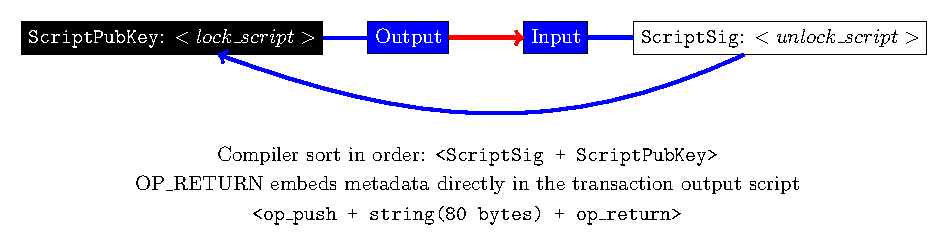
\includegraphics[scale=0.5]{figures/script.pdf}
\end{frame}


\begin{frame}{Literature Review}
    \framesubtitle{OP\_RETURN}
OP\_RETURN is the most widely used mechanism for anchoring non-monetary data in Bitcoin.
It is adopted by protocols such as Blockcerts~\cite{Blockcerts} and OpenTimestamps~\cite{OpenTimestamps}.\\
\vspace*{0.2cm}
However, OP\_RETURN-based approaches exhibit several limitations:
\begin{itemize}
    \item Embedded data is explicitly visible on-chain, limiting privacy.
    \item Data capacity per transaction is constrained by policy and fee costs.
    \item Merkle-based aggregation is not enforced at the protocol level and must be implemented out protocol.
\end{itemize}
\end{frame}

\begin{frame}{Literature Review}
    \framesubtitle{SegWit}
Kedziora et al.~\cite{Kedziora2022AnalysisSegWit} analyze the impact of the Segregated Witness (SegWit) soft fork after its deployment.\\
\vspace*{0.2cm}
SegWit separates signature data from the transaction body into a dedicated witness structure, improving efficiency and security.\\
\vspace*{0.2cm}
This design resolves transaction malleability and reduces effective transaction cost.\\
\vspace*{0.2cm}
Additionally, anchoring data via the witness allows larger payloads without increasing UTXO set growth.\\
\centering
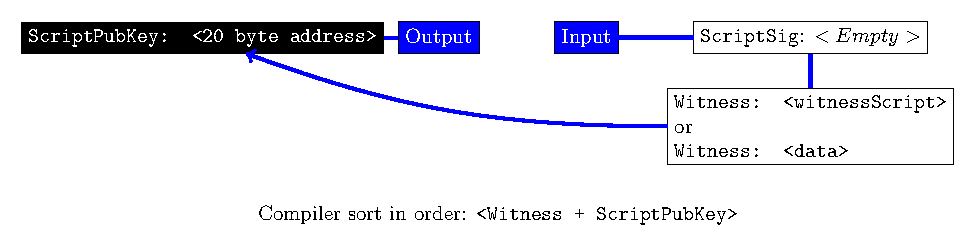
\includegraphics[scale=0.6]{figures/witness.pdf}
\end{frame}


\begin{frame}{Literature Review}
    \framesubtitle{Solutions in Alternative Blockchains}
Several works, including Wang~\cite{Wang2019BlockchainCT}, Li~\cite{Li2020DecentralizedPKI}, Pennino~\cite{Pennino2021EfficientCertification}, Palmisano~\cite{Palmisano2022NotarizationAntiPlagiarism}, Mishra~\cite{Mishra2025BlockchainDecentralized}, and Harer~\cite{Harer2022DecentralizedAttestation}, leverage smart contracts on Ethereum to attest information such as certificates, timestamps, and structured data.\\
\vspace*{0.2cm}
These works show that:
\begin{itemize}
    \item Smart contracts enable expressive and flexible certification logic.
    \item On-chain execution incurs high operational costs due to gas fees.
    \item Increased programmability introduces implementation complexity and security risks.
\end{itemize}
\end{frame}

\begin{frame}{Literature Review}
    \framesubtitle{Example: Solutions for Academic Organizations}
The work \emph{Blockchain and Higher Education Diplomas}~\cite{Castro2021BlockchainHigherEducation} notes that, as a radical innovation, blockchain adoption in academic contexts must overcome both technical barriers (scalability, error correction, system complexity) and cultural or social barriers (lack of standards and resistance to change).\\
\vspace*{0.2cm}
A systematic literature review by Rustemi et al.~\cite{Rustemi2023SLRBlockchainCertificates} identifies that most existing academic certificate verification platforms are implemented on Ethereum and rely on smart contracts for service execution.
\begin{block}{Remark}
Verification can be performed autonomously, while certificate issuance and revocation remain challenging and often require third-party involvement.
\end{block}
\end{frame}


\begin{frame}{Literature Review}
    \framesubtitle{New Cryptographic Tools}
Bitcoin has evolved its protocol to improve security, privacy, and efficiency, with SegWit resolving transaction vulnerabilities~\cite{segwit}.\\
\vspace*{0.2cm}
Building on these foundations, Taproot integrates Schnorr signatures and Merkleized Abstract Syntax Trees (MAST), which have been extensively studied in the literature~\cite{Gayoso2020AnalysisCryptographic,Fang2020DigitalSignature,Zhang2025HighEfficiencySchnorrMultiSignature}.\\
\vspace*{0.2cm}
These cryptographic tools form the basis of the Taproot soft fork specified in BIP341, extending SegWit with more efficient and private spending conditions~\cite{taproot}.\\
\vspace*{0.2cm}
Taproot introduces a new transaction output type, Pay-to-Taproot (P2TR), activated on the Bitcoin network in November 2021.\\
\vspace*{0.2cm}
This upgrade expands the design space for Bitcoin-native applications at the base layer.
\end{frame}


\begin{frame}{Literature Review}
    \framesubtitle{Gap Identified}
To the best of our knowledge, a complete Taproot-based protocol for decentralized document verification on Bitcoin has not been systematically studied.\\
\vspace*{0.3cm}
Taproot provides:
\begin{itemize}
    \item Improved privacy and efficiency through hidden script paths.
    \item Native support for compact commitments and batching via MAST.
\end{itemize}
\end{frame}
